% -*- Mode:TeX -*-

%% IMPORTANT: There are no official thesis specifications.
%%            This unofficial thesis specifications are available at:
%%            https://github.com/ikenichiro/KeioSDM_phdtmp
%%
%%            The original format and specifications are from mit,
%%            which can be found at:
%%            http://libraries.mit.edu/archives/thesis-specs/
%%
%%            Please verify your thesis' formatting and copyright
%%            assignment before submission. If you notice any
%%            discrepancies between these templates and the
%%            Keio Universitys' specs, please let me know
%%            from the github issue.

%% The documentclass options along with the pagestyle can be used to generate
%% a technical report, a draft copy, or a regular thesis.  You may need to
%% re-specify the pagestyle after you \include  cover.tex.  For more
%% information, see the first few lines of keiosdmthesis.cls. 

%\documentclass[12pt,vi,twoside]{keiosdmthesis}
%%
%%  If you want your thesis copyright to you instead of Keio University, use the
%%  ``vi'' option, as above.
%%
%\documentclass[12pt,twoside,leftblank]{keiosdmthesis}
%%
%% If you want blank pages before new chapters to be labelled ``This
%% Page Intentionally Left Blank'', use the ``leftblank'' option, as
%% above.
%\RequirePackage{pdf14}
\documentclass[12pt,vi,twoside]{keiosdmthesis}
\usepackage{lgrind}
%% These have been added at the request of the MIT Libraries, because
%% some PDF conversions mess up the ligatures.  -LB, 1/22/2014
\usepackage{cmap}
\usepackage[T1]{fontenc}
\pagestyle{plain}

%% These have been added to use pdf figures
\usepackage{epsfig} \let\epsfile=\epsfig%
\usepackage{epic,eepic}
\usepackage[dvipdfmx]{color}

%% Some commonly used packages.
%\usepackage{cleveref}
%\usepackage{amsmath,amssymb}
%\usepackage{etoolbox}
%\usepackage{booktabs}
%\usepackage{color}
%\usepackage{url}
%\usepackage{siunitx}
%
%% These have been added for glossaries
%\usepackage[nonumberlist,acronym,toc]{glossaries}
%% These are for trademark but usage of trademark in academic thesis are not recommended.
%\usepackage{textcomp} 
%
%\usepackage{listings}
%\usepackage{multirow}
%\usepackage[figuresright]{rotating}
%\usepackage[flushleft]{threeparttable}
%\usepackage{comment}
%
%\usepackage[dvipdfmx,bookmarks=true]{hyperref}
%% This is a hyperref hack to make it work at the least with emath.
%% Be sure this comes after all of the \usepackage
%\AtBeginDocument{\let\textlabel\label}%

%% This allows to label in the text so it can cross-ref from Appendix easily.
%% Try considering cleveref from the start of your thesis.
%% This hack was done on the last minutes just to adapt to cleveref in aux.
%% Original code can be found at,
%% https://tex.stackexchange.com/questions/271062/labeling-a-text-and-referencing-it-later
%% Usage:
%% \labelText{}{a:ch1:labelname}
%% type out by:
%% \cref{a:ch1:labelname}
%\newcounter{mylabelcounter}
%\makeatletter
%\newcommand{\labelText}[2]{%
%  #1\refstepcounter{mylabelcounter}%
%  \immediate\write\@auxout{%
%  %make it accessable from cref
%    \string\newlabel{#2}{{1}{\thepage}{{\unexpanded{#1}}}{mylabelcounter.\number\value{mylabelcounter}}{}}%
%  }
%  \immediate\write\@auxout{%
%    \string\newlabel{#2@cref}{{[page][\thepage]}{\thepage}}%
%  }%
%}
\makeatother
%% Ends here

%% This bit allows you to either specify only the files which you wish to
%% process, or `all' to process all files which you \include.
%% Krishna Sethuraman (1990).

%\typein [\files]{Enter file names to process, (chap1,chap2 ...), or `all' to process all files:}
%\typein[\files]{chap1}
%\def\all{all}
%\ifx\files\all \typeout{Including all files.} \else \typeout{Including only \files.} \includeonly{\files} \fi
%\includeonly{chap1,chap2}

%% Define the sort mode for bibliography
\bibliographystyle{junsrt}
%% Rename the title for bibliography
\renewcommand{\bibname}{List of References}

%% Define glossaries
%% Generate list of symbols
%\newglossary[slg]{symbols}{syi}{syg}{List of symbols}
%% Remove the dot at the end of glossary descriptions
%\renewcommand*{\glspostdescription}{}
%\makeglossaries%
%% Load nomenclature and glossary files
%\loadglsentries{nomenclature}
%\loadglsentries{glossary} %Acronyms here

%%setup for siunitx
%\sisetup{binary-units,per-mode=symbol}

\begin{document}
%% Set page numbering as roman until the thesis actually starts
\pagenumbering{roman}
\setcounter{page}{1}

% -*-latex-*-
%
% For questions, comments, concerns or complaints:
% https://github.com/ikenichiro/KeioSDM_phdtmp
% 
% --- Original statements --- 
% For questions, comments, concerns or complaints:
% thesis@mit.edu
% 
%
% $Log: cover.tex,v $
% Revnote
% Make the covermode definable from preamble (like vi mode)
%
% Revision 1.8  2008/05/13 15:02:15  jdreed
% Degree month is June, not May.  Added note about prevdegrees.
% Arthur Smith's title updated
%
% Revision 1.7  2001/02/08 18:53:16  boojum
% changed some \newpages to \cleardoublepages
%
% Revision 1.6  1999/10/21 14:49:31  boojum
% changed comment referring to documentstyle
%
% Revision 1.5  1999/10/21 14:39:04  boojum
% *** empty log message ***
%
% Revision 1.4  1997/04/18  17:54:10  othomas
% added page numbers on abstract and cover, and made 1 abstract
% page the default rather than 2.  (anne hunter tells me this
% is the new institute standard.)
%
% Revision 1.4  1997/04/18  17:54:10  othomas
% added page numbers on abstract and cover, and made 1 abstract
% page the default rather than 2.  (anne hunter tells me this
% is the new institute standard.)
%
% Revision 1.3  93/05/17  17:06:29  starflt
% Added acknowledgements section (suggested by tompalka)
% 
% Revision 1.2  92/04/22  13:13:13  epeisach
% Fixes for 1991 course 6 requirements
% Phrase "and to grant others the right to do so" has been added to 
% permission clause
% Second copy of abstract is not counted as separate pages so numbering works
% out
% 
% Revision 1.1  92/04/22  13:08:20  epeisach

% NOTE:
% These templates make an effort to conform to the MIT Thesis specifications,
% however the specifications can change.  We recommend that you verify the
% layout of your title page with your thesis advisor and/or the MIT 
% Libraries before printing your final copy.
\title{Unofficial thesis template for Graduate School of Keio University System Design and Management}

\author{Keio Taro}
% If you wish to list your previous degrees on the cover page, use the 
% previous degrees command:
%       \prevdegrees{A.A., Harvard University (1985)}
% You can use the \\ command to list multiple previous degrees
%       \prevdegrees{B.S., University of California (1978) \\
%                    S.M., Massachusetts Institute of Technology (1981)}
\department{Graduate School of System Design and Management}

% If the thesis is for two degrees simultaneously, list them both
% separated by \and like this:
% \degree{Doctor of Philosophy \and Master of Science}
\degree{Ph.D. in System Engineering}
%\degree{Ph.D. in System Design and Management}

% As of the 2007-08 academic year, valid degree months are September, 
% February, or June.  The default is June.
\degreemonth{March}
\degreeyear{2017}
\thesisdate{March, 23 2017} % Please check if the date is correct each year.

%% By default, the thesis will be copyrighted to KeioSDM.  If you need to copyright
%% the thesis to yourself, just specify the `vi' documentclass option.  If for
%% some reason you want to exactly specify the copyright notice text, you can
%% use the \copyrightnoticetext command.  
%\copyrightnoticetext{\copyright Keio Taro, 2017.}

% If there is more than one supervisor, use the \supervisor command
% once for each.
\supervisor{Keio Taro}{Professor, Department of System Design and Management}

% This is the department committee chairman, not the thesis committee
% chairman.  You should replace this with your Department's Committee
% Chairman.
\chairman{Keio Hanako}{Chairman, Department of System Design and Management} % Takeshi Maeno 

% Make the titlepage based on the above information.  If you need
% something special and can't use the standard form, you can specify
% the exact text of the titlepage yourself.  Put it in a titlepage
% environment and leave blank lines where you want vertical space.
% The spaces will be adjusted to fill the entire page.  The dotted
% lines for the signatures are made with the \signature command.
\maketitle

% The abstractpage environment sets up everything on the page except
% the text itself.  The title and other header material are put at the
% top of the page, and the supervisors are listed at the bottom.  A
% new page is begun both before and after.  Of course, an abstract may
% be more than one page itself.  If you need more control over the
% format of the page, you can use the abstract environment, which puts
% the word "Abstract" at the beginning and single spaces its text.

%% You can either \input (*not* \include) your abstract file, or you can put
%% the text of the abstract directly between the \begin{abstractpage} and
%% \end{abstractpage} commands.

% First copy: start a new page, and save the page number.
\cleardoublepage%
% Uncomment the next line if you do NOT want a page number on your
% abstract and acknowledgments pages.
\pagestyle{empty}
%\setcounter{savepage}{\thepage}
\begin{abstractpage}
\addcontentsline{toc}{chapter}{Abstract}
% Consider the readability!
% https://www.online-utility.org/english/readability_test_and_improve.jsp
write abstract here.


\end{abstractpage}

% Additional copy: start a new page, and reset the page number.  This way,
% the second copy of the abstract is not counted as separate pages.
% Uncomment the next 6 lines if you need two copies of the abstract
% page.
% \setcounter{page}{\thesavepage}
% \begin{abstractpage}
% % Consider the readability!
% https://www.online-utility.org/english/readability_test_and_improve.jsp
write abstract here.


% \end{abstractpage}

\cleardoublepage%

\section*{Acknowledgments}
\addcontentsline{toc}{chapter}{Acknowledgments}
Write thanks here.
Many people also like to thank their parents and family.
Lastly, I would like to thank my parents and my relatives for their faithful support.
%%%%%%%%%%%%%%%%%%%%%%%%%%%%%%%%%%%%%%%%%%%%%%%%%%%%%%%%%%%%%%%%%%%%%%
% -*-latex-*-

%% Some departments require an additional signature page.
%% See signature.tex for more information and uncomment the following line if applicable.
% -*- Mode:TeX -*-
% This is used in KeioSDM template.
%
% Some departments (e.g. Chemistry) require an additional cover page
% with signatures of the thesis committee.  Please check with your
% thesis advisor or other appropriate person to determine if such a 
% page is required for your thesis.  
%
% If you choose not to use the "titlepage" environment, a \newpage
% commands, and several \vspace{\fill} commands may be necessary to
% achieve the required spacing.  The \signature command is defined in
% the "mitthesis" class
%
% The following sample appears courtesy of Ben Kaduk <kaduk@mit.edu> and
% was used in his June 2012 doctoral thesis in Chemistry. 

\begin{titlepage}
\begin{large}
This doctoral thesis has been examined by a Committee of the Graduate School of System Design and Management as follows:

\signature{Professor Taro Keio}{Chairman, Thesis Supervisor \\
   Professor of System Design and Management}

\signature{Professor Hanako System}{Member, Thesis Committee \\
   Professor of System Design and Management}

\signature{Professor Jiro Design}{Member, Thesis Committee \\
   Professor of System Design and Management}

\signature{Professor Kusako Management}{Member, Thesis Committee \\
   Professor of Information Systems at the University of Elsewhere}

\signature{Doctor Saburo Company}{Member, Thesis Committee \\
   Doctor of Engineering, Some Corportaion}

 \end{large}
\end{titlepage}


\pagestyle{plain}
%% This is to make Table of Contents
% -*- Mode:TeX -*-
%% This file simply contains the commands that actually generate the table of
%% contents and lists of figures and tables.  You can omit any or all of
%% these files by simply taking out the appropriate command.  For more
%% information on these files, see appendix C.3.3 of the LaTeX manual. 
\setcounter{secnumdepth}{4}
\setcounter{tocdepth}{4}
\tableofcontents
\newpage
\listoffigures
\newpage
\listoftables
\newpage

%% Start page count in arabic after Table of Contents
\pagenumbering{arabic}
\setcounter{page}{1}
\chapter{Introduction}\label{ch1:intro}
Sample Introduction.
In this introduction, Section~\ref{ch1:back} describes about the research background.
Section~\ref{ch1:purpose} describes about the research purpose, and Section~\ref{ch1:outline} will describe the structure of this dissertation.

\section{Background}\label{ch1:back}
Write research background here.

\subsection{Subsection of background}\label{ch1:subback}
Sample cite\cite{sample:2001} shown in sample Figure~\ref{fig:fig1.1_1} refs.
\begin{figure}[!b]
  \centering 
  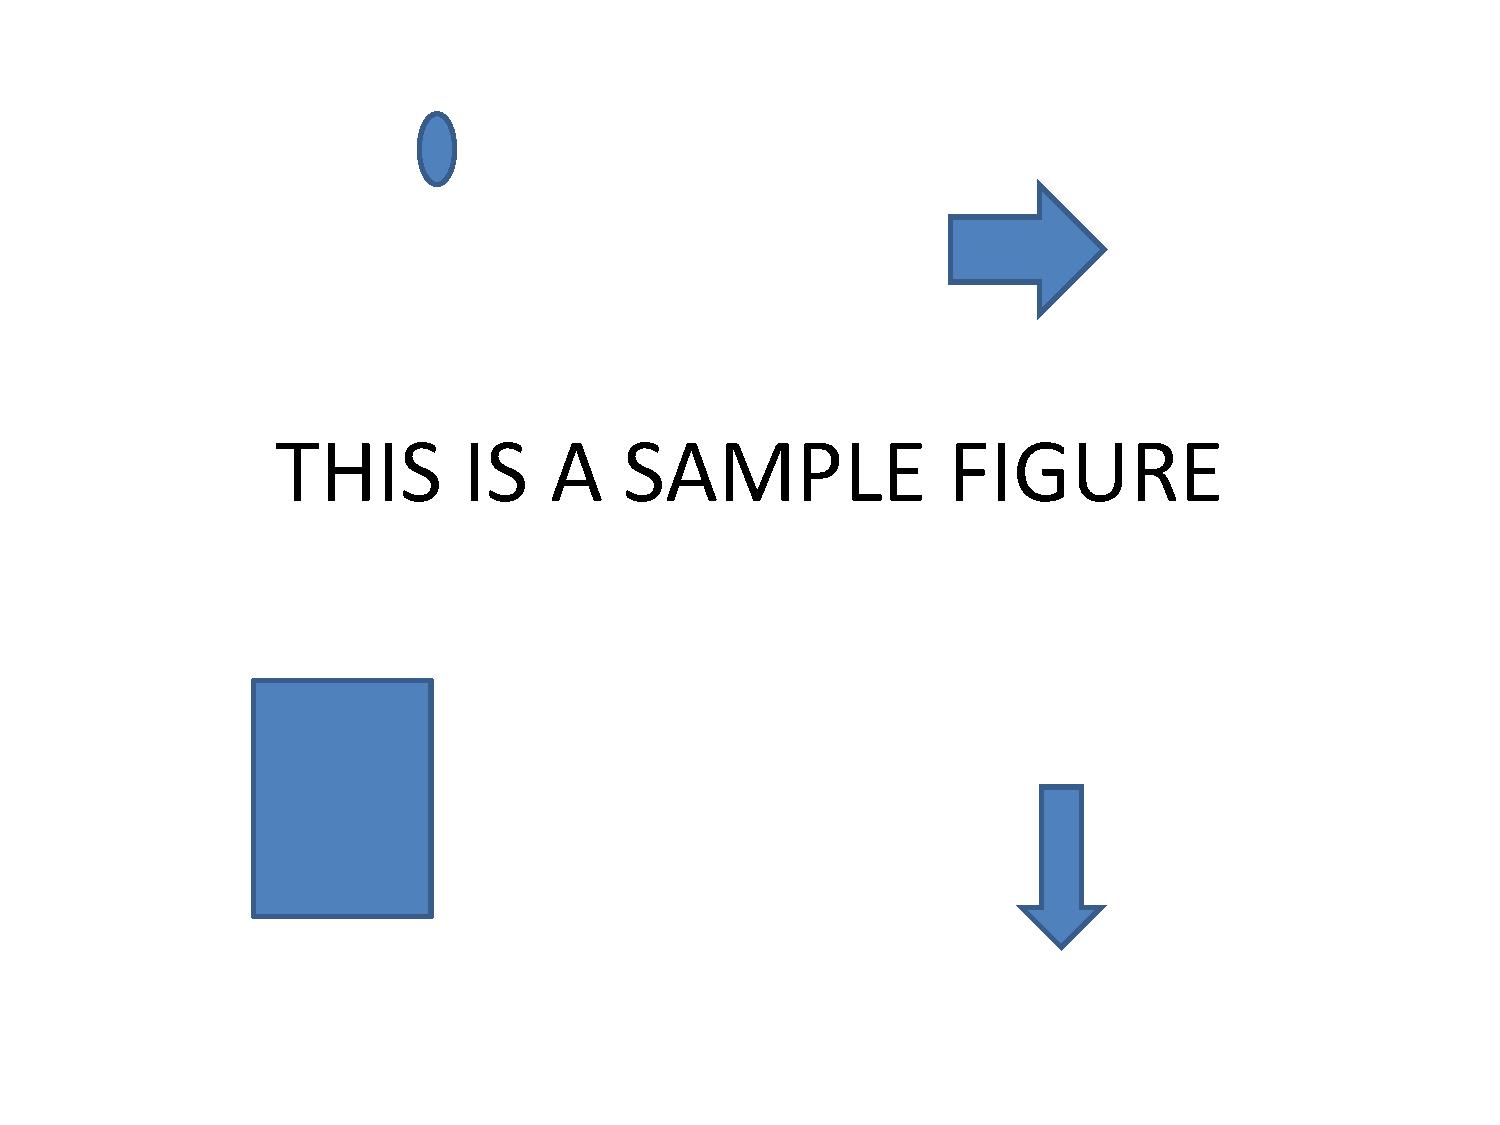
\includegraphics[width=0.5\textwidth,keepaspectratio]{{{Figures/fig1.1_1sample}}}
  \caption[Short caption for TOC.]{This is normal long caption you can write to describe in long figure caption sentence.}\label{fig:fig1.1_1}%
\end{figure}

\section{Research Purpose}\label{ch1:purpose}
Sample research purpose.

\section{Research Outline}\label{ch1:outline}
The remainder of this dissertation is organized as follows.

Chapter~\ref{ch2:sample} focus on how some sample.

Chapter~\ref{ch3:sample} describes about more samples.

Chapter~\ref{ch4:sample} concludes this dissertation.
Finally, limitations of this research and possible research foresights will be briefly explained.

Figure~\ref{fig:1.3_1sample} illustrates the outline of this dissertation.
\begin{figure}[!b]
  \centering%
    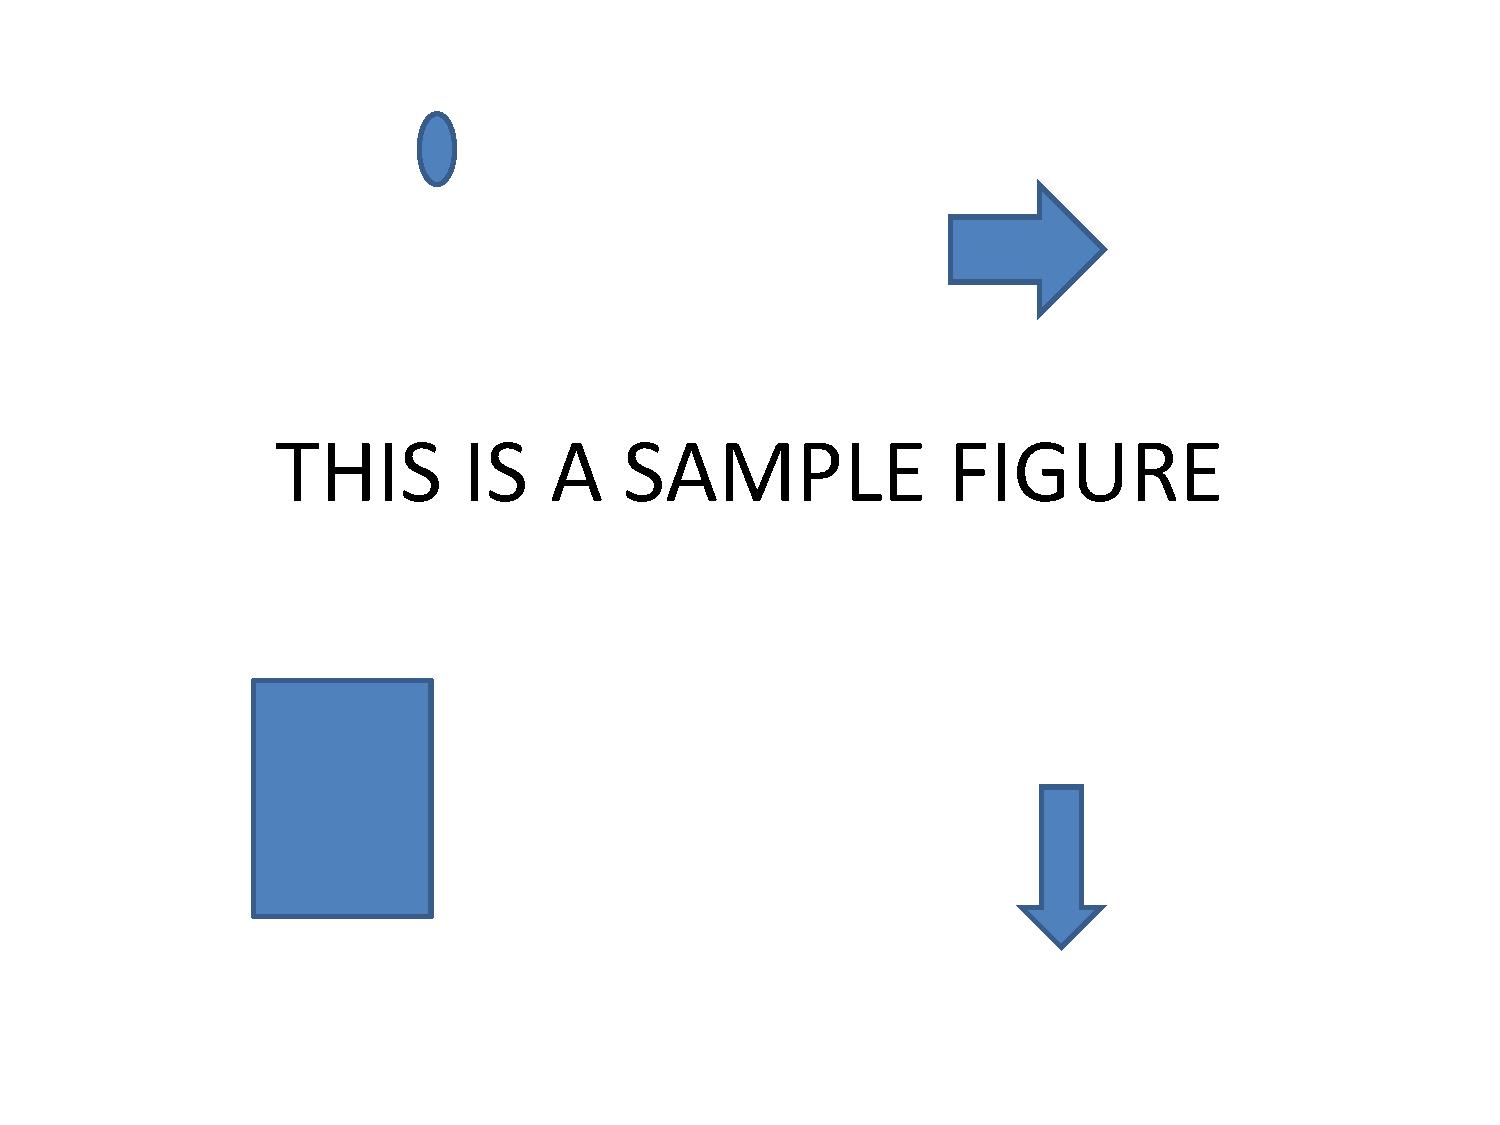
\includegraphics[width=\textwidth,keepaspectratio]{{{Figures/fig1.3_1_to}}}
    \caption{Short caption only one.}\label{fig:1.3_1sample}%
\end{figure}


\chapter{sample of the second chapter}\label{ch2:sample}
This is the sample of the second chapter of this template.


\chapter{The third sample}\label{ch3:sample}
This is the third sample chapter.

\chapter{The forth sample}\label{ch4:sample}
This is the forth sample chapter.

\appendix
%% Appendix Tables
\chapter{Tables}

\begin{table}
\caption{Armadillos}
\label{arm:table}
\begin{center}
\begin{tabular}{||l|l||}\hline
Armadillos & are \\\hline
our	   & friends \\\hline
\end{tabular}
\end{center}
\end{table}

\clearpage
\newpage

%% Appendix Figures and Codes
\chapter{Figures}

\vspace*{-3in}

\begin{figure}
\vspace{2.4in}
\caption{Armadillo slaying lawyer.}
\label{arm:fig1}
\end{figure}
\clearpage
\newpage

\begin{figure}
\vspace{2.4in}
\caption{Armadillo eradicating national debt.}
\label{arm:fig2}
\end{figure}
\clearpage
\newpage

%% List of symbols, nomenclature, glossary
%% Print the glossary
%\printglossary[style=altlist,title=Glossary]
%% Print list of acronyms
%\printglossary[type=\acronymtype,style=long,title=Acronyms]
%% Print list of symbols
%\printglossary[type=symbols,style=long4col]
%\clearpage


%% List of bibliography
%% This defines the bibliography file (main.bib) and the bibliography style.
%% If you want to create a bibliography file by hand, change the contents of
%% this file to a `thebibliography' environment.  For more information 
%% see section 4.3 of the LaTeX manual.
\begin{singlespace}
  \addcontentsline{toc}{chapter}{List of References}
  \bibliography{bib_ref,bib_mywork} % this reads the 0_ref.bib and mywork.bib
\bibliographystyle{plain}
\end{singlespace}

%% List of related publications
% method from stackexchange.com
% https://tex.stackexchange.com/questions/97057/including-additional-bibliography-publication-list-in-thesis
\begin{singlespace}
  \addcontentsline{toc}{chapter}{List of Publications}
  \chapter*{List of Publications}
  List of related publications.
  \begin{center}
    \textbf{Refereed Journal Publications}
  \end{center}
  \begin{itemize}
    \item
      \underline{\bfseries Taro Keio}, Hanako System, Jiro Design and Kusako Management.
      \newblock Journal title comes here.
      \newblock {\em Transactions of the Keio SDM (in Japanese)}, Vol.~1, No. 1, pp.1--11.
      \newblock in Japanese.

    \item
      \underline{\bfseries Taro Keio}, Hanako System, Jiro Design and Kusako Management.
      \newblock Journal title comes here.
      \newblock {\em Transactions of the LaTeX Templates}, Vol.~1, No. 1, pp.1--11.
  \end{itemize}
  \begin{center}
    \textbf{Refereed Full Papers in Conference Proceedings}
  \end{center}
  \begin{itemize}
    \item
      \underline{\bfseries Taro Keio} and Hanako System.
      \newblock Title of the proceedings comes here.
      \newblock In {\em LaTeX Template Proceedings} {\em Sample Conference 2013}. Sample Conference on LaTeX Template, September 2013., pp.1--13

    \item
      \underline{\bfseries Taro Keio} and Hanako System.
      \newblock Title of the proceedings comes here.
      \newblock In {\em LaTeX Template Proceedings} {\em Sample Conference 2015}. Sample Conference on LaTeX Template, August 2015., pp.1--13
  \end{itemize}

  \begin{center}
    \textbf{Refereed Works in Conference (Demos and Posters)}
  \end{center}
  \begin{itemize}
    \item \textbf{(Poster)}
      \underline{\bfseries Taro Keio} and Hanako System.
      \newblock Title of the poster comes here.
      \newblock In {\em LaTeX Template Conference} {\em Sample Conference 2014}. Sample Conference on LaTeX Template, July 2014., pp.100--102

    \item \textbf{(Demo)}
      \underline{\bfseries Taro Keio} and Hanako System.
      \newblock Title of the poster comes here.
      \newblock In {\em LaTeX Template Conference} {\em Sample Conference 2012}. Sample Conference on LaTeX Template, July 2012., pp.90--92
  \end{itemize}

  \begin{center}
    \textbf{Non-refereed Conference Paper}
  \end{center}
  \begin{itemize}
    \item
      \underline{\bfseries Taro Keio} and Hanako System.
      \newblock Title of the proceedings comes here.
      \newblock In {\em Sample Report (in Japanese)} {\em 20th Conference on Sample Conference}, Vol.~1. Sample Society of Japan, June 2013., pp. 49--61.
      \newblock in Japanese.

  \end{itemize}

  \begin{center}
    \textbf{Non-first Author Publications}
  \end{center}
  \begin{itemize}
    \item
      Hanako System and \underline{Taro Keio}.
      \newblock Some title comes here.
      \newblock In {\em Sample conference (in Japanese)} {\em 4th Conference on Sample Conference}, Vol.~1. Sample Society of Japan, June 2011., pp. 54--66.
      
  \end{itemize}

  \begin{center}
    \textbf{Others}
  \end{center}
  \begin{itemize}
    \item
      \underline{\bfseries Kenichiro Ito}.
      \newblock If any put in the title.
      \newblock Invited Presentation at some other something.

  \end{itemize}
\end{singlespace}

\end{document}

